\documentclass[convert=pdf2svg,multi=false]{standalone}
\usepackage{tikz}
  \usetikzlibrary{positioning}
\begin{document}
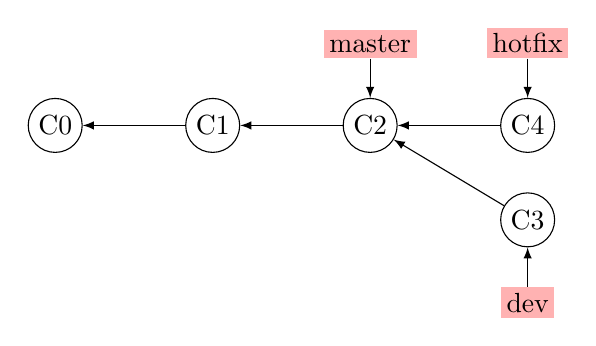
\begin{tikzpicture}[commit/.style={draw,circle,inner sep=2pt},pointer/.style={draw=none,fill=red!30,rectangle,inner sep=2pt}]
\foreach \i[count=\x] in {0,1,2,4} {
   \node[commit] (C\i) at (2*\x,0) {C\i};
}
\node[commit, below=.5 of C4] (C3) {C3};
\foreach \i/\j in {0/1,1/2,2/3,2/4} {
  \draw[latex-] (C\i) -- (C\j);
}
\node[pointer] (master) [above=.5 of C2] {master};
\node[pointer] (dev) [below=.5 of C3] {dev};
\node[pointer] (hotfix) [above=.5 of C4] {hotfix};
\draw[-latex] (master) -- (C2);
\draw[-latex] (dev) -- (C3);
\draw[-latex] (hotfix) -- (C4);
\end{tikzpicture}
\end{document}